% #############################################################################
% This is Appendix A
% !TEX root = ../main.tex
% #############################################################################
\chapter{Benchmark Results}
\label{chapter:appendixResults}

This appendix contains the full benchmark results that were summarized in \Cref{chap:evaluation}. The source code for the benchmarks is too large to include in this document, but is available in the GitHub repository\footnote{\url{https://github.com/RiscadoA/class}} containing the implementation of the compiler and the runtime system. The programs used for the benchmarks were the prime sieve, at \texttt{examples/sam/sam-sieve-sum-fast-stop-intp.clls}, the Game of Life, at \texttt{tests/complex/game\_of\_life\_2.clls}, and finally, the shared queue, which can be found at \texttt{examples/LFCS/xqueue-n.clls}.

Each of the benchmarks was run 10 times for each data point, and the average execution time and memory usage were recorded. The execution time and memory usage were measured using the GNU \texttt{time -v} command, which provides detailed information about the resources used by a program. The maximum \acf{RSS} was used as the measure of memory usage. All results were obtained on a machine with an Intel Core i9-12900K CPU and 32GB of RAM, running NixOS 25.05.

To measure the impact of each implemented optimization, multiple compiler configurations were tested. The \texttt{base} configuration has all optimizations disabled, except for the exponential value optimization, which is not configurable. The \texttt{optimized} configuration has all optimizations enabled. The rest of the configurations are split into two groups: the \texttt{<set>} configurations which have only the specified optimizations enabled, and the \texttt{no-<set>} configurations which have all optimizations enabled except for the specified one. The benchmarked optimization sets are described below:
\begin{itemize}[noitemsep, topsep=0pt, partopsep=0pt, parsep=0pt, labelindent=0pt]
    \item \texttt{inlining}: Inlining and monomorphization of process calls.
    \item \texttt{values}: Enables the optimizations which change the representation of sends of value types and affine types, as described in \Cref{subsection:SendValueOptimizations,subsection:AffineValueOptimizations}.
    \item \texttt{endpoints}: Enables tail calls, uses symbolic execution to find and eliminate redundant exit points, and avoids branching on processes with a single exit point, as described in \Cref{section:SingleExitPointOptimizations,section:IRSimplification}.
    \item \texttt{control-flow}: Uses symbolic execution to find and eliminate known jumps, branches and always set drop bits, as described in \Cref{section:IRSimplification}.
    \item \texttt{locations}: Replaces data locations referring to known continuations with direct data locations, as described in \Cref{section:IRSimplification}.
\end{itemize}

The Haskell implementation of the benchmarks was compiled using GHC 9.8.4 with the \texttt{-O2} optimization flag.

\clearpage
\section{Prime sieve results}

\begin{figure}[H]
    \centering
    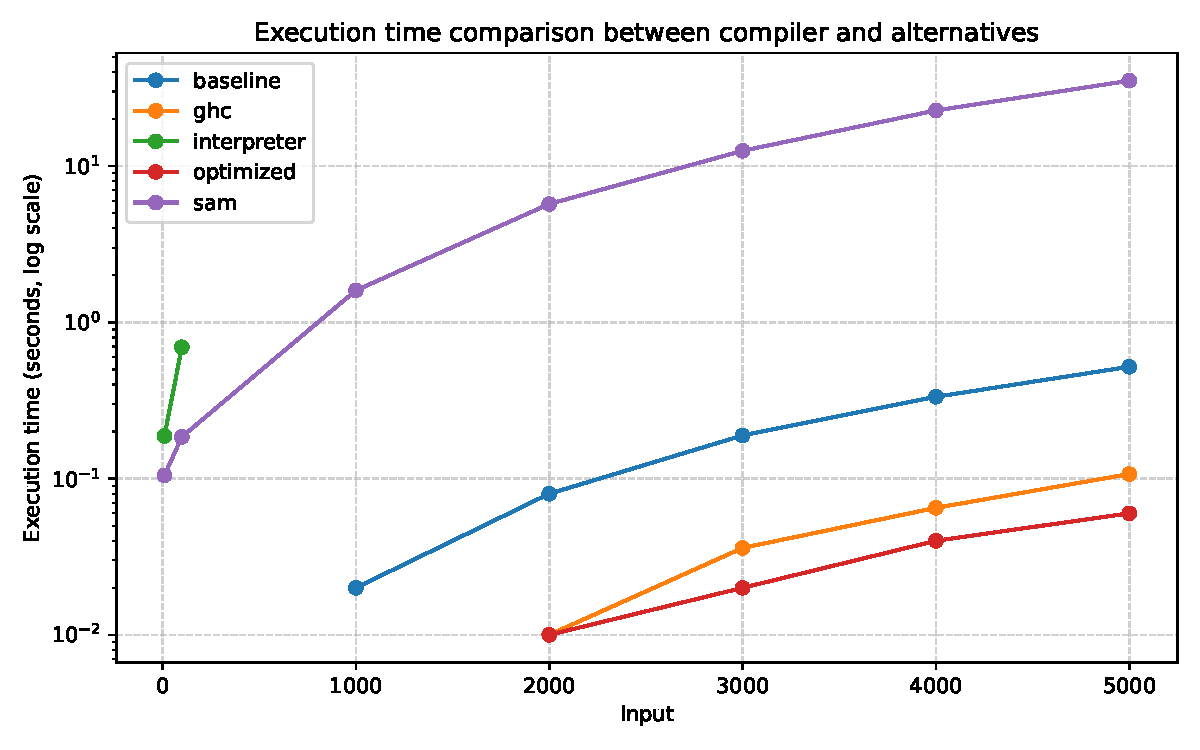
\includegraphics[width=0.49\textwidth]{./Images/execution_time_sieve_compiler_vs_alternatives.pdf}
    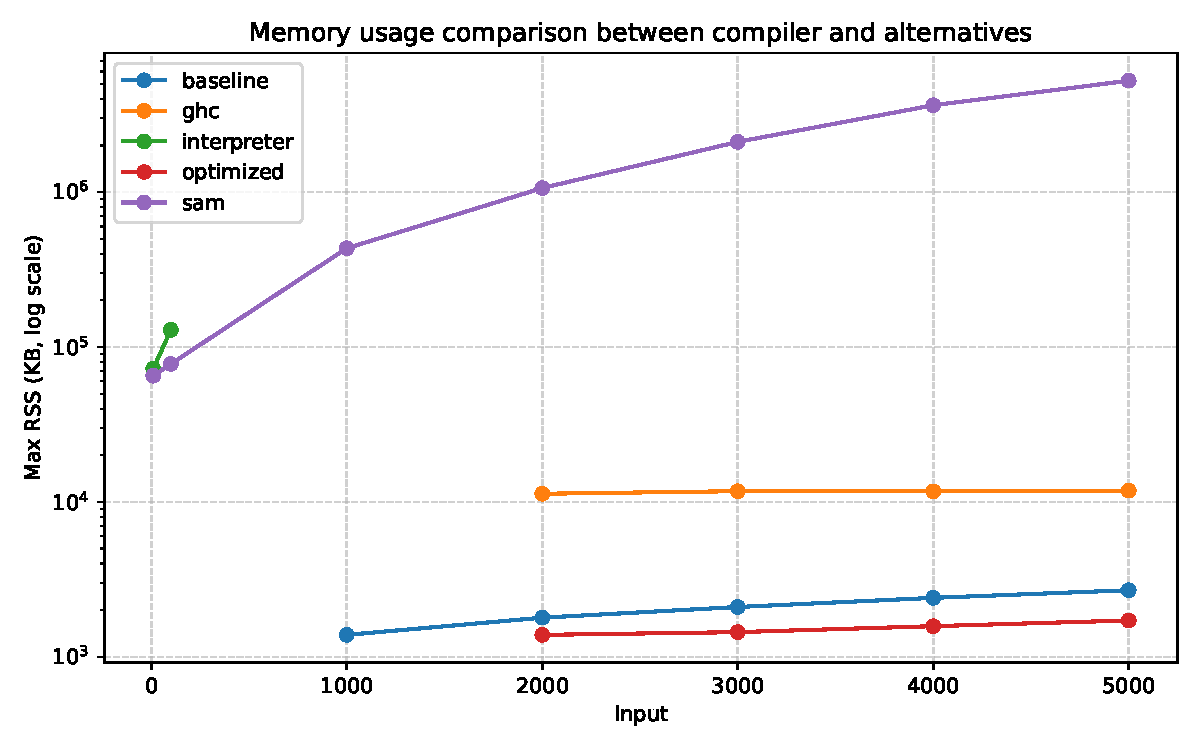
\includegraphics[width=0.49\textwidth]{./Images/memory_usage_sieve_compiler_vs_alternatives.pdf}
    \captionof{figure}{Same as \Cref{fig:SieveBenchmarkCompilerVsAlternatives} (repeated for reference). Compares the prime sieve benchmarks across the original interpreter, the SAM, the baseline compiler, the compiler with all optimizations enabled, and GHC.}
\end{figure}
\begin{figure}[H]
    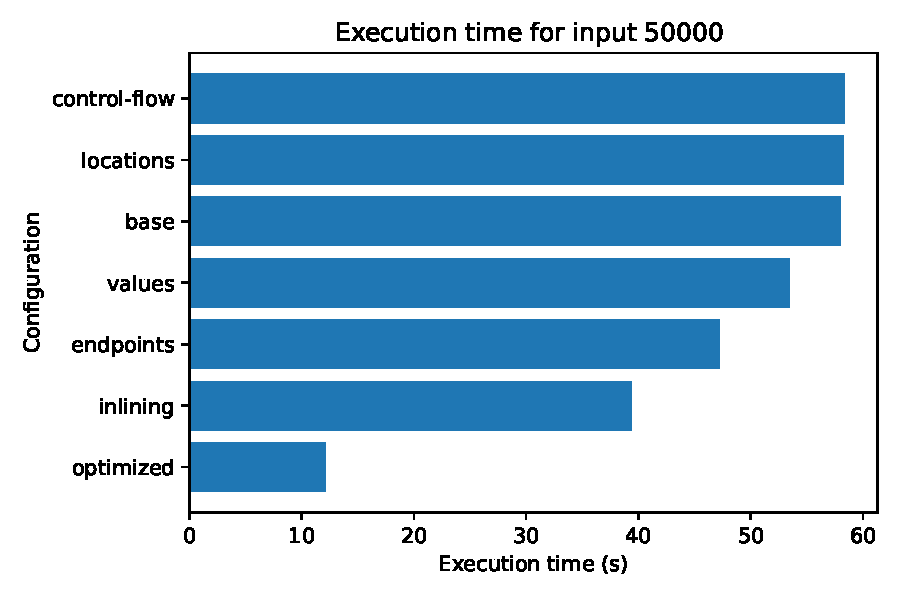
\includegraphics[width=0.49\textwidth]{./Images/execution_time_sieve_enabled_opts.pdf}
    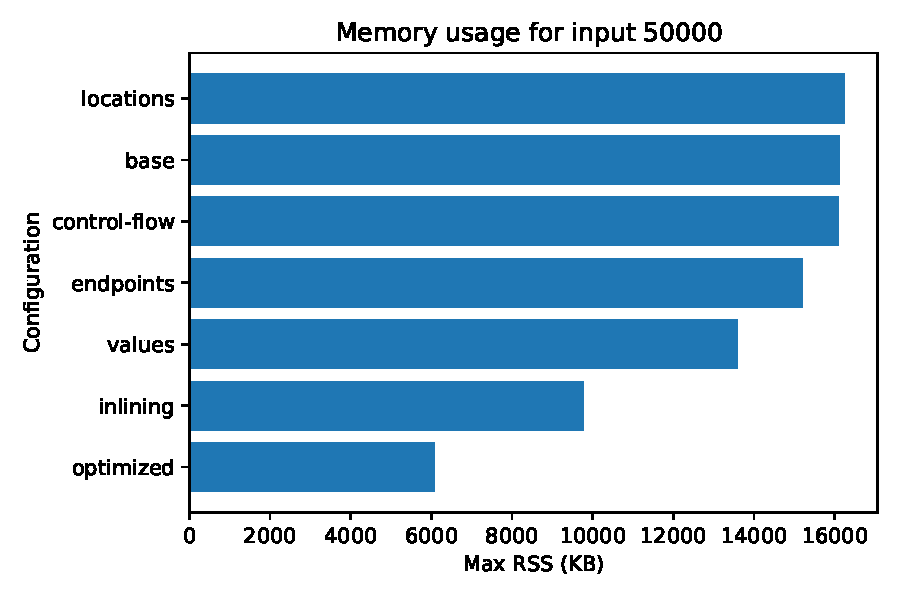
\includegraphics[width=0.49\textwidth]{./Images/memory_usage_sieve_enabled_opts.pdf}
    \caption{Prime sieve benchmarks averaged over 10 runs, with a fixed prime count of 50000. Compares the baseline compiler, the fully optimized compiler, and multiple compiler configurations with only specific optimizations enabled.}
    \label{fig:SieveBenchmarkTimeAcrossConfigurations}
\end{figure}
\begin{figure}[H]
    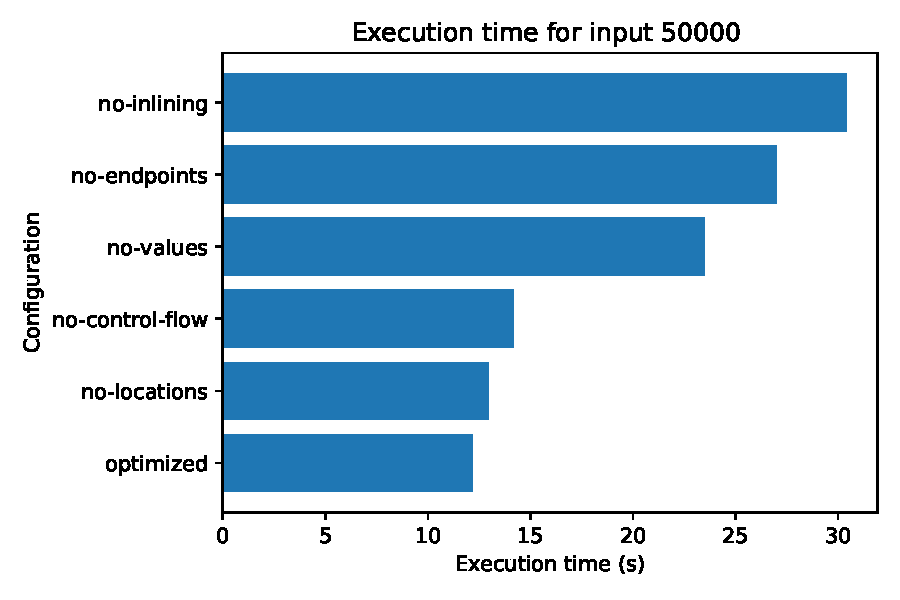
\includegraphics[width=0.49\textwidth]{./Images/execution_time_sieve_disabled_opts.pdf}
    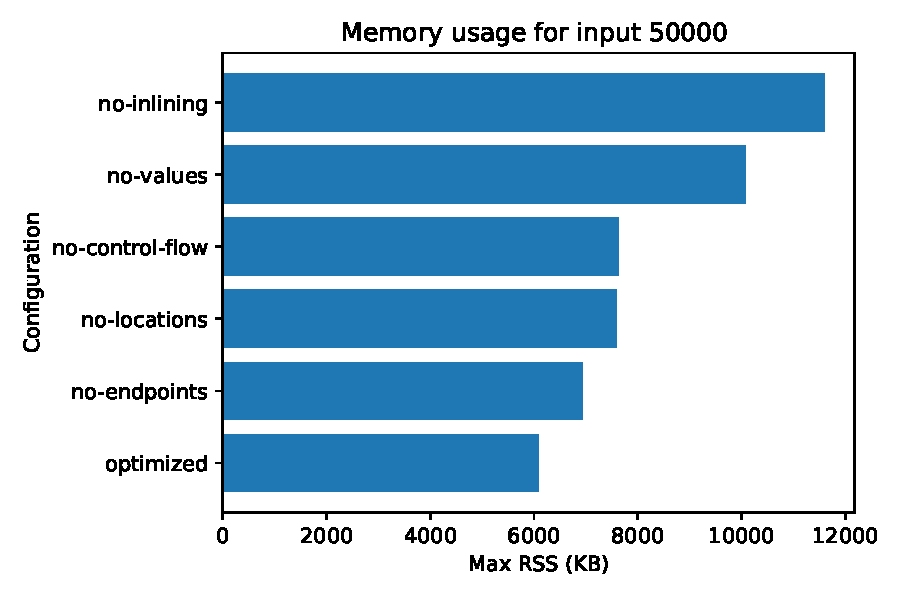
\includegraphics[width=0.49\textwidth]{./Images/memory_usage_sieve_disabled_opts.pdf}
    \caption{Prime sieve benchmarks averaged over 10 runs, with a fixed prime count of 50000. Compares the fully optimized compiler, and multiple compiler configurations with only specific optimizations disabled.}
    \label{fig:SieveBenchmarkMemoryAcrossConfigurations}
\end{figure}

\section{Game of Life results}

\begin{figure}[H]
    \centering
    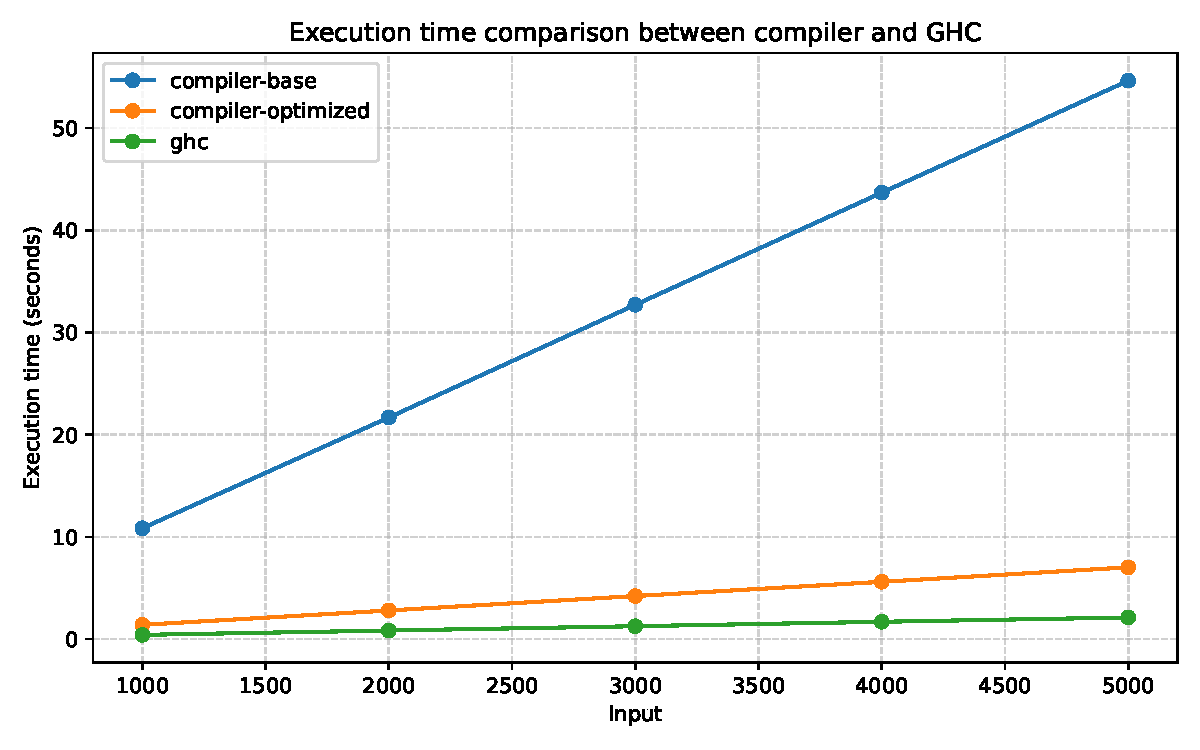
\includegraphics[width=0.49\textwidth]{./Images/execution_time_gol_compiler_vs_ghc.pdf}
    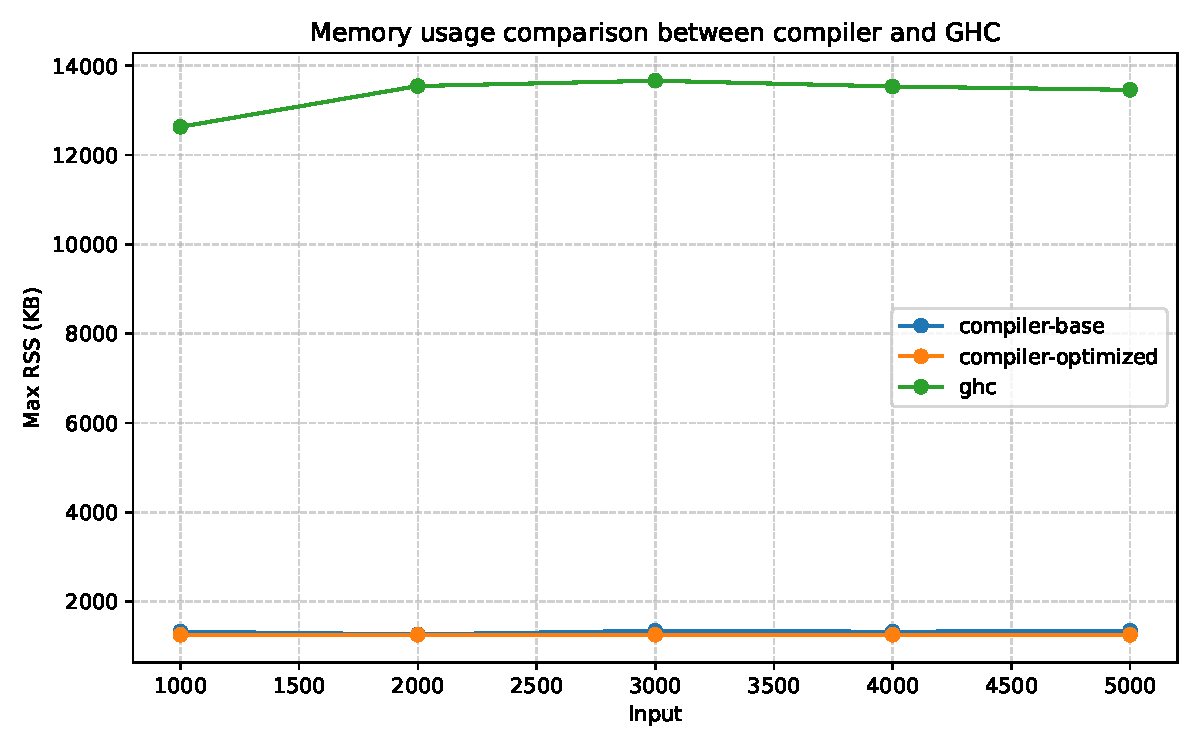
\includegraphics[width=0.49\textwidth]{./Images/memory_usage_gol_compiler_vs_ghc.pdf}
    \captionof{figure}{Same as \Cref{fig:GOLBenchmarkCompilerVsGHC} (repeated for reference). Compares the Game of Life benchmarks across the baseline compiler, the compiler with all optimizations enabled, and GHC.}
\end{figure}
\begin{figure}[H]
    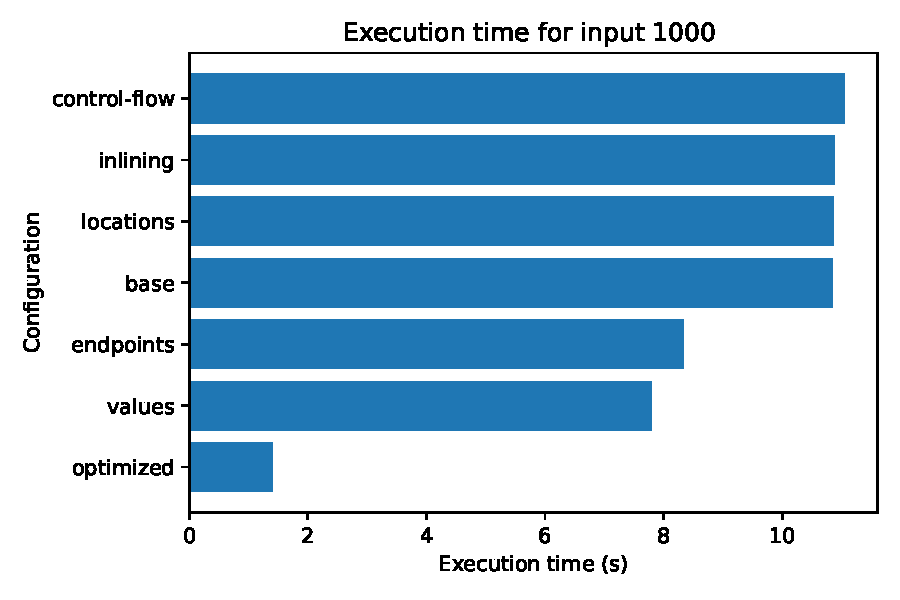
\includegraphics[width=0.49\textwidth]{./Images/execution_time_gol_enabled_opts.pdf}
    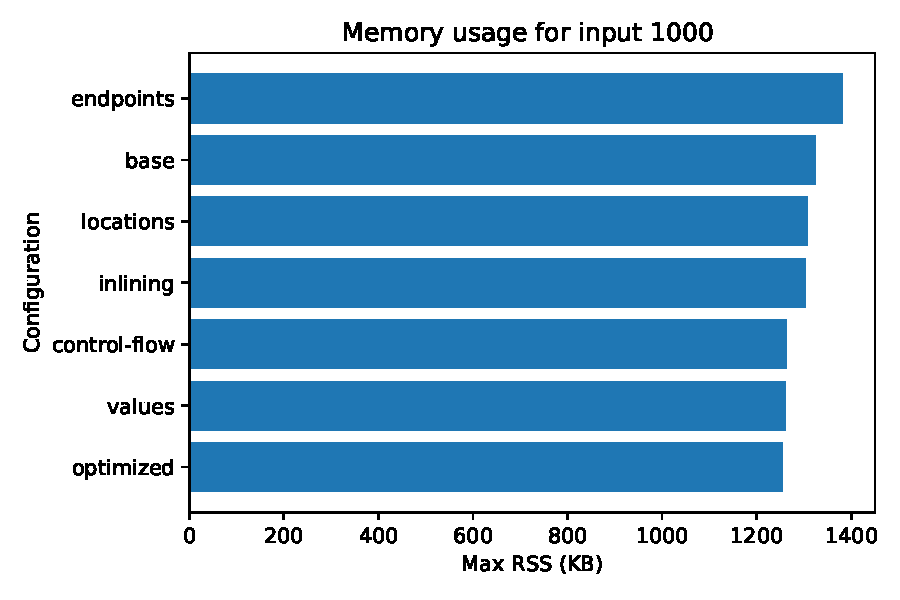
\includegraphics[width=0.49\textwidth]{./Images/memory_usage_gol_enabled_opts.pdf}
    \caption{Game of Life benchmarks averaged over 10 runs, with a fixed generation count of 1000. Compares the baseline compiler, the fully optimized compiler, and with only specific optimizations enabled.}
    \label{fig:GOLBenchmarkTimeAcrossConfigurations}
\end{figure}
\begin{figure}[H]
    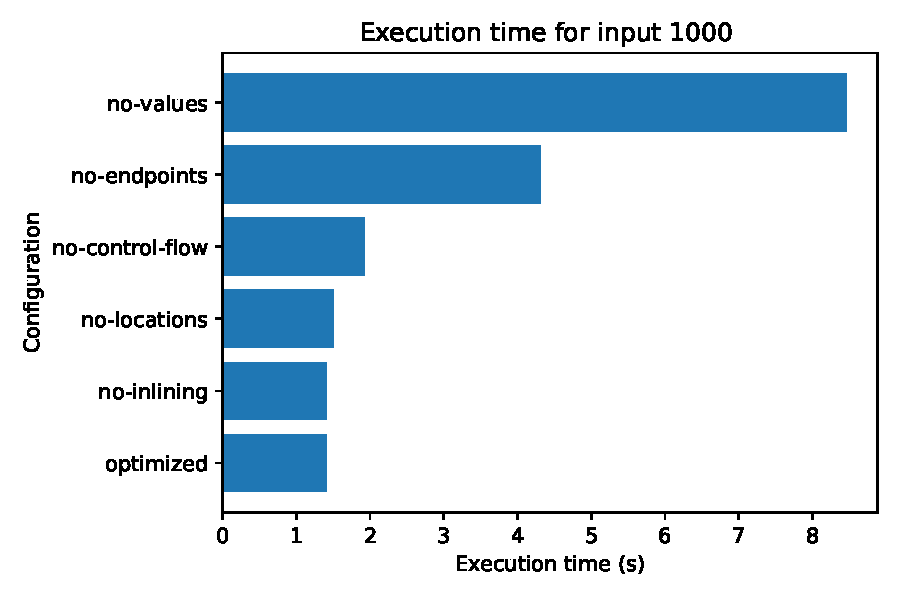
\includegraphics[width=0.49\textwidth]{./Images/execution_time_gol_disabled_opts.pdf}
    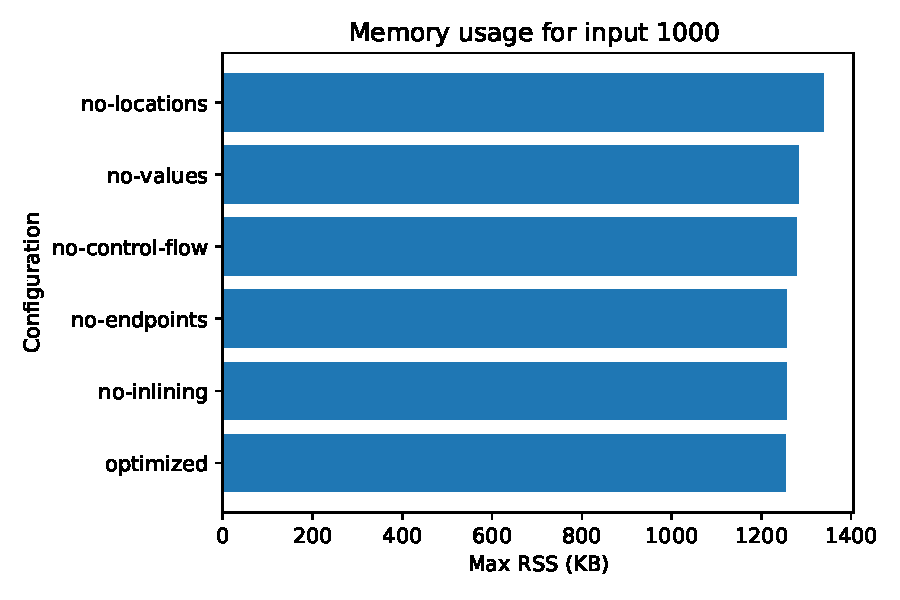
\includegraphics[width=0.49\textwidth]{./Images/memory_usage_gol_disabled_opts.pdf}
    \caption{Game of Life benchmarks averaged over 10 runs, with a fixed generation count of 1000. Compares the fully optimized compiler, and multiple compiler configurations with only specific optimizations disabled.}
    \label{fig:GOLBenchmarkMemoryAcrossConfigurations}
\end{figure}

\section{Shared queue results}

\begin{figure}[H]
    \centering
    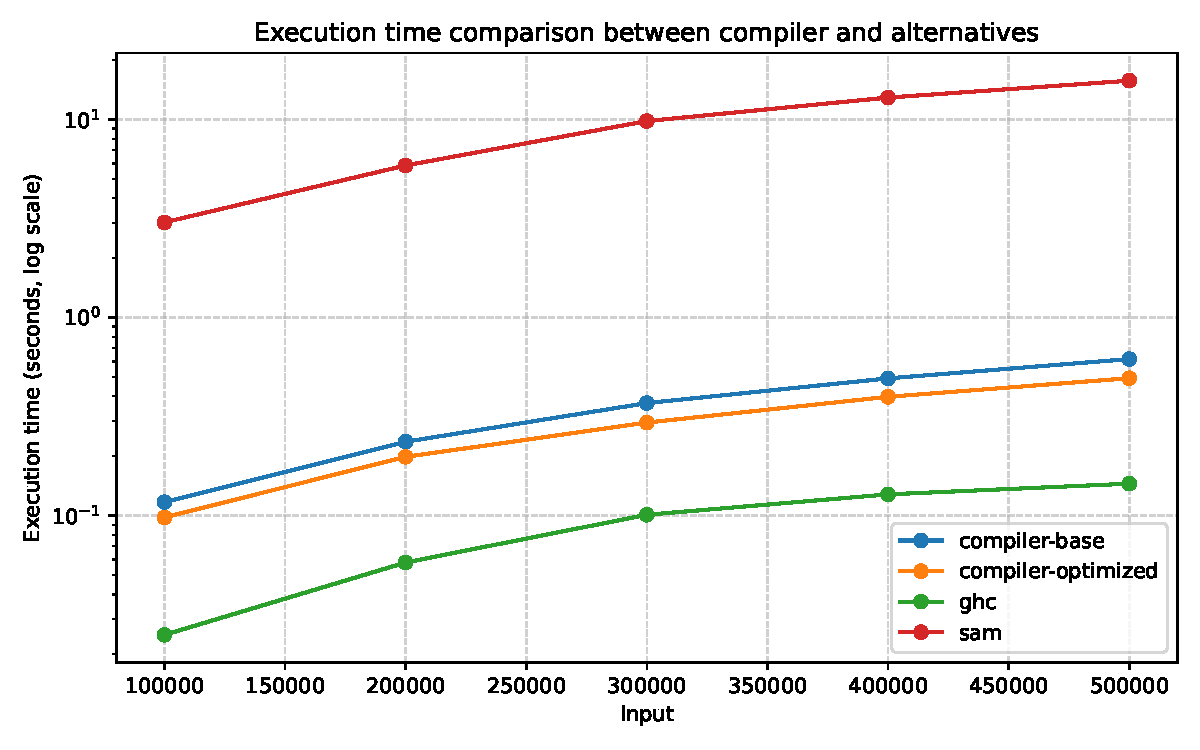
\includegraphics[width=0.49\textwidth]{./Images/execution_time_queue_compiler_vs_alternatives.pdf}
    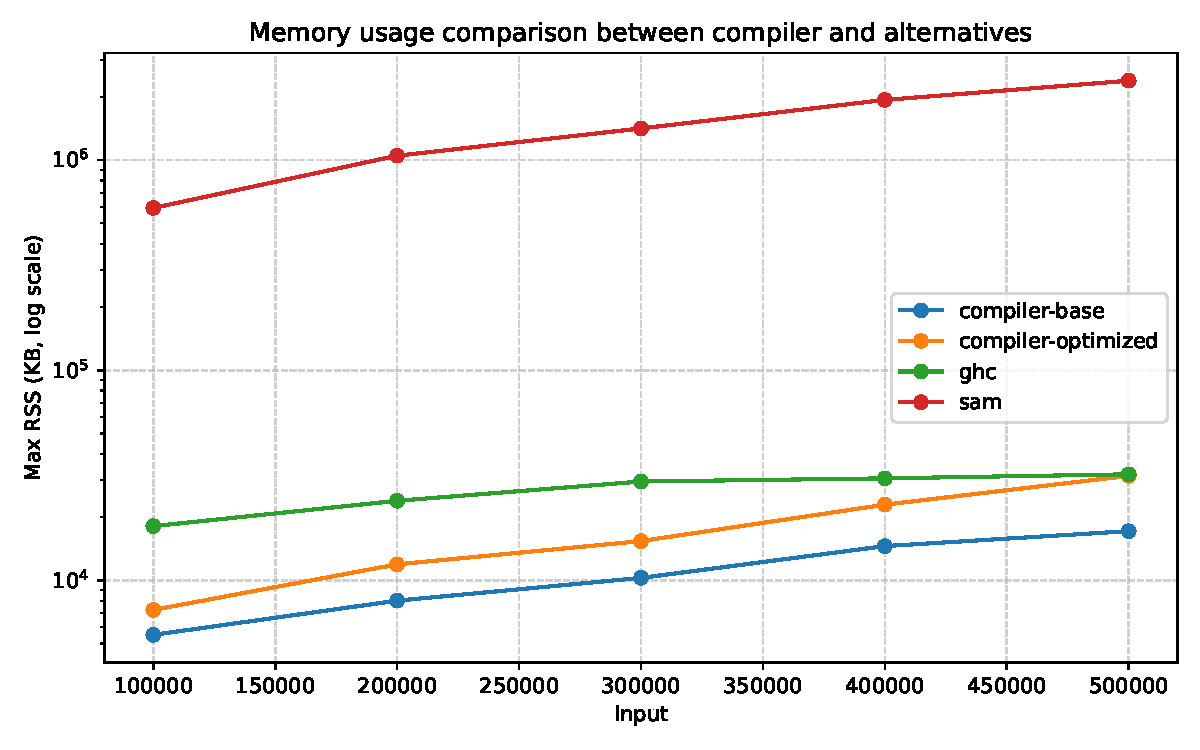
\includegraphics[width=0.49\textwidth]{./Images/memory_usage_queue_compiler_vs_alternatives.pdf}
    \caption{Shared queue benchmarks averaged over 10 runs, parametrized over item count. Compares the SAM, the baseline compiler, the compiler with all optimizations enabled, and GHC. The original interpreter was were unable to run this benchmark.}
    \label{fig:QueueBenchmarkCompilerVsAlternatives}
\end{figure}
\begin{figure}[H]
    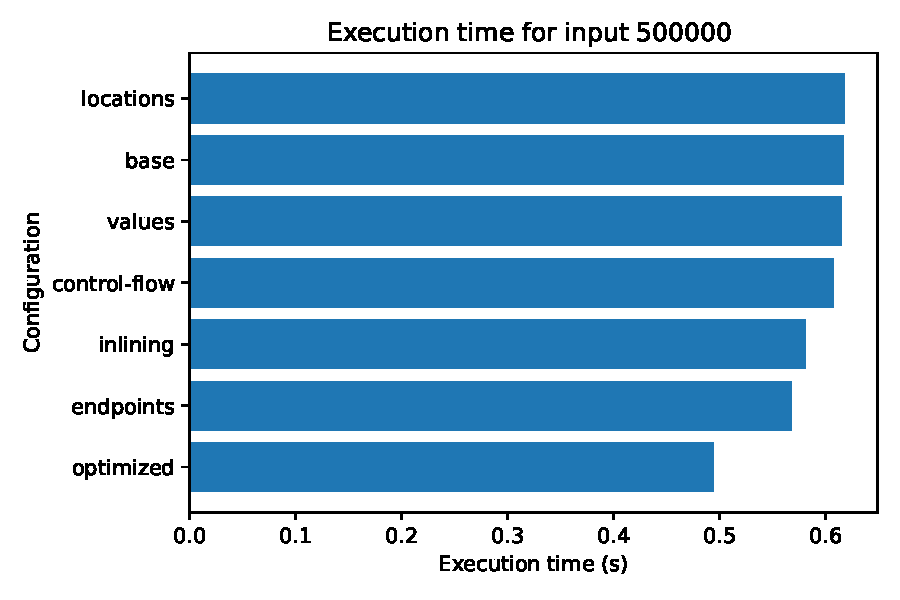
\includegraphics[width=0.49\textwidth]{./Images/execution_time_queue_enabled_opts.pdf}
    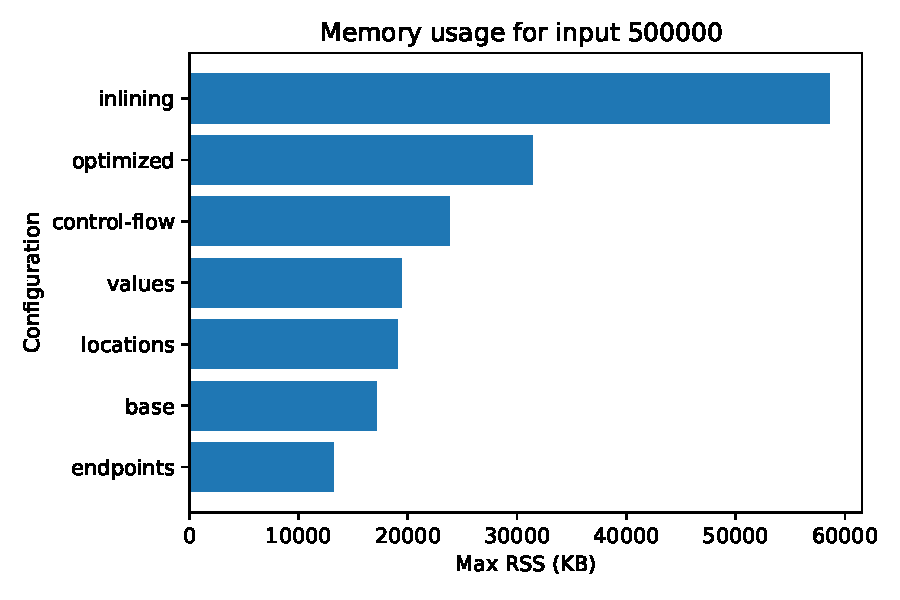
\includegraphics[width=0.49\textwidth]{./Images/memory_usage_queue_enabled_opts.pdf}
    \caption{Shared queue benchmarks averaged over 10 runs, with a fixed item count of 500000. Compares the baseline compiler, the fully optimized compiler, and with only specific optimizations enabled.}
    \label{fig:QueueBenchmarkTimeAcrossConfigurations}
\end{figure}
\begin{figure}[H]
    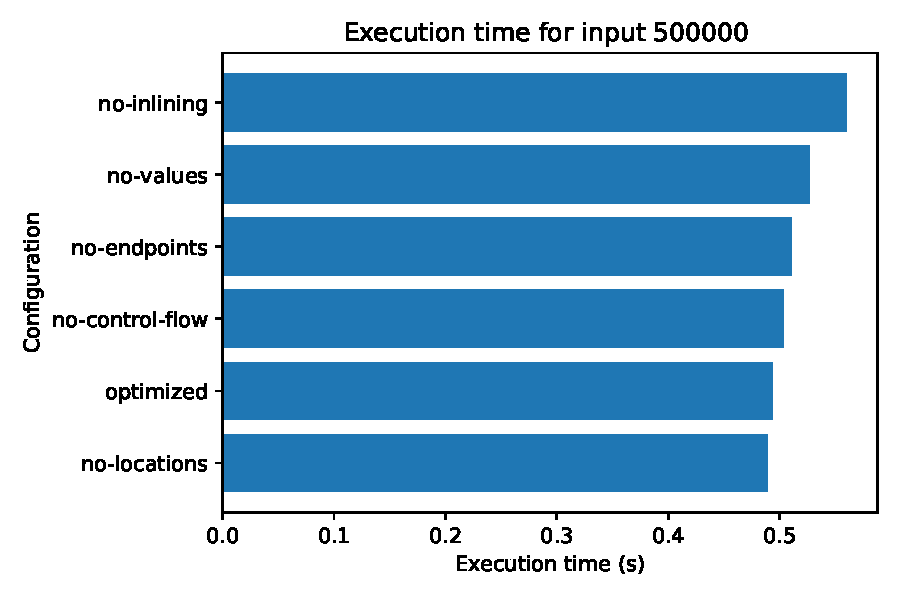
\includegraphics[width=0.49\textwidth]{./Images/execution_time_queue_disabled_opts.pdf}
    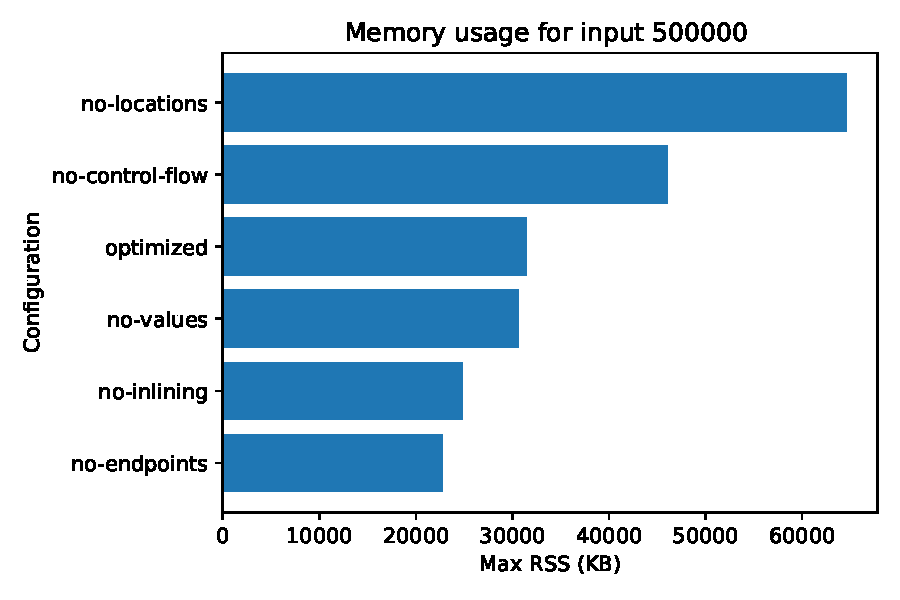
\includegraphics[width=0.49\textwidth]{./Images/memory_usage_queue_disabled_opts.pdf}
    \caption{Shared queue benchmarks averaged over 10 runs, with a fixed item count of 500000. Compares the fully optimized compiler, and multiple compiler configurations with only specific optimizations disabled.}
\label{fig:QueueBenchmarkMemoryAcrossConfigurations}
\end{figure}
